\documentclass[12pt]{article}


\usepackage{amssymb}
\usepackage{amsmath}
\usepackage{fullpage}
\usepackage{epsfig}
\usepackage{epstopdf}
\everymath{\displaystyle}

\newif\ifans

\ansfalse

\begin{document}

\begin{center}
\underline{\LARGE{Area Between Two Curves}}
\end{center}

\noindent SUGGESTED REFERENCE MATERIAL:

\bigskip

\noindent As you work through the problems listed below, you should reference Chapter 6.1 of the recommended textbook (or the equivalent chapter in your alternative textbook/online resource) and your lecture notes.

\bigskip

\noindent EXPECTED SKILLS:

\begin{itemize}

\item Be able to find the area between the graphs of two functions over an interval of interest.

\item Know how to find the area enclosed by two graphs which intersect.

\end{itemize}

\noindent PRACTICE PROBLEMS:

\medskip

\begin{enumerate}

\item Let $R$ be the shaded region shown below.

\begin{center}

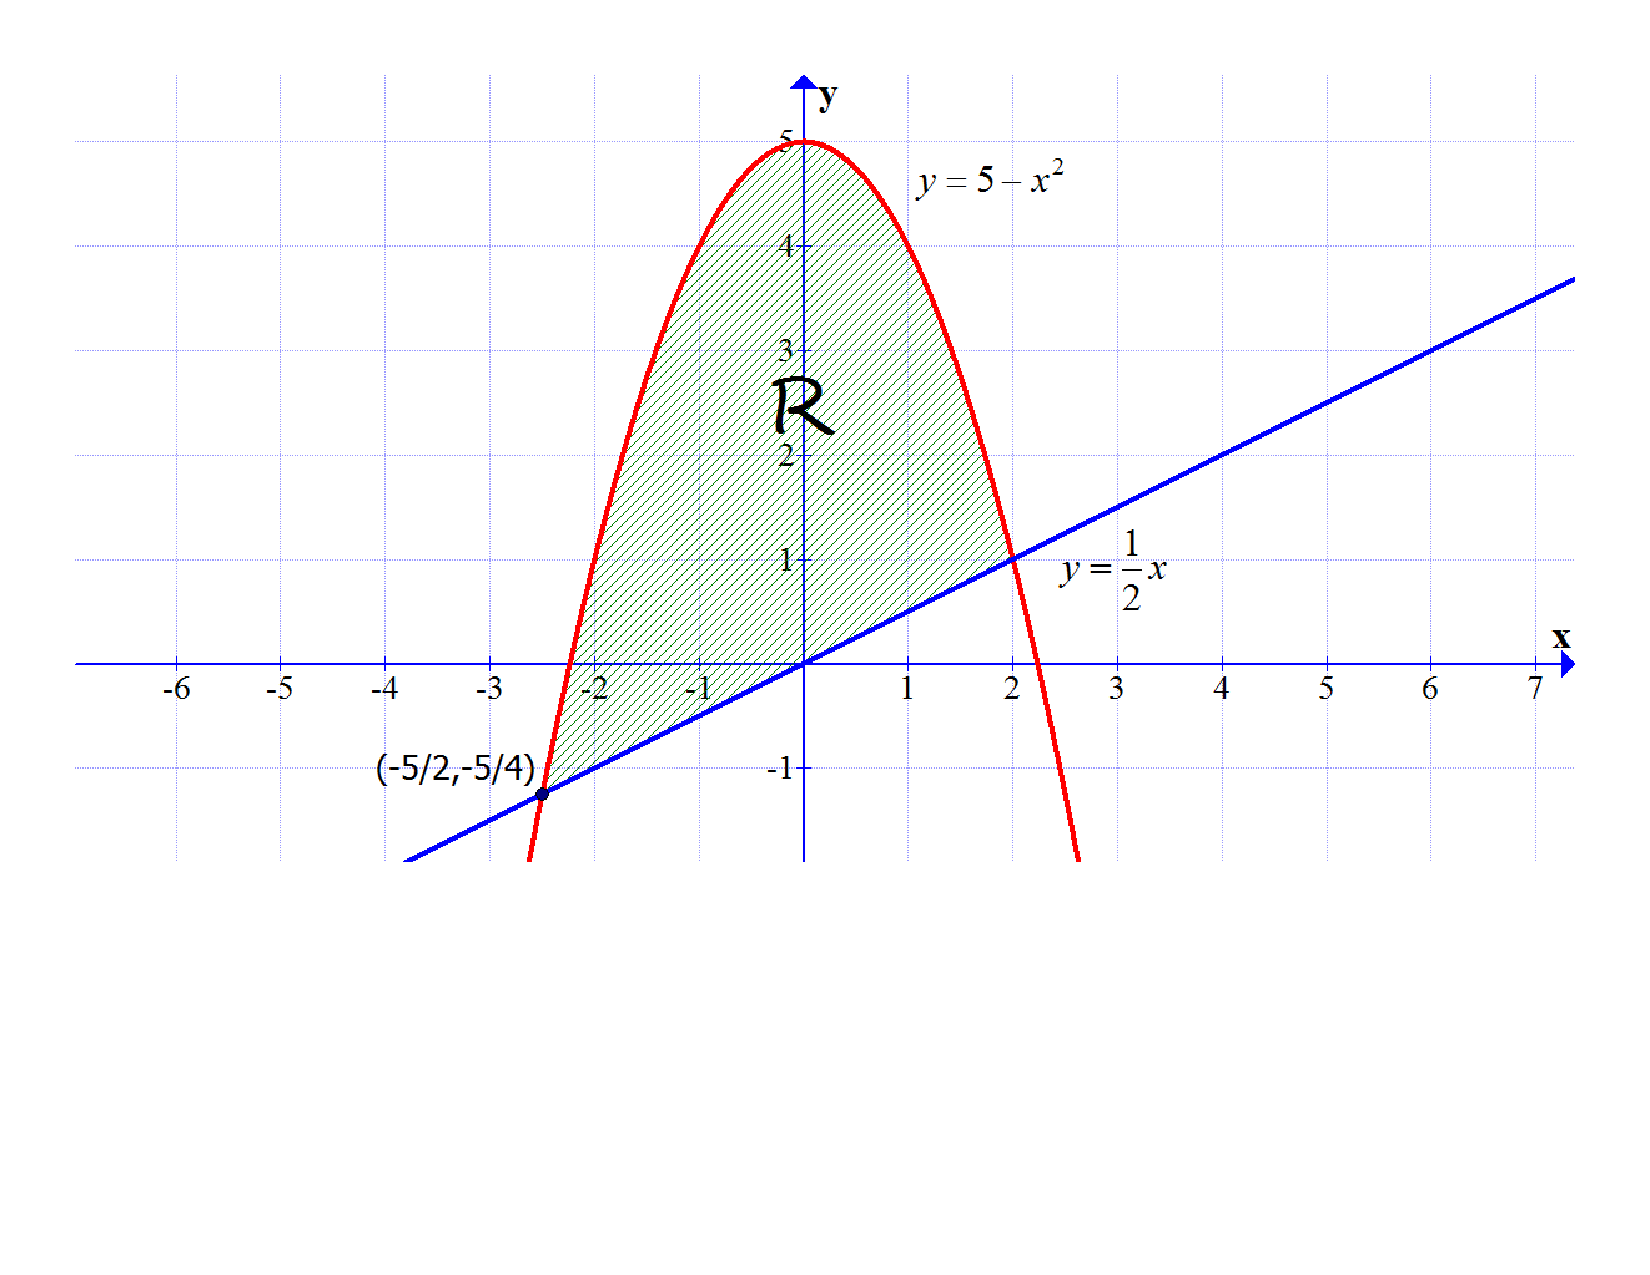
\includegraphics[scale=0.5]{graph3.pdf}

\end{center}

\begin{enumerate} 

\item Set up but do not evaluate an integral (or integrals) \underline{in terms of $x$} that represent(s) the area of $R$. 

\ifans{\fbox{$\int_{-\frac{5}{2}}^2 \left(-x^2-\frac{1}{2}x+5\right) \,dx$}} \fi

\item Set up but do not evaluate an integral (or integrals) \underline{in terms of $y$} that represent(s) the area of $R$. 

\ifans{\fbox{$\int_{-\frac{5}{4}}^1 \left(2y+\sqrt{5-y}\right) \,dy+2\int_1^5 \sqrt{5-y} \,dy$}} \fi

\end{enumerate}

\end{enumerate}

\newpage

\noindent {\bf For problems 2-4, compute the area of the shaded region.}

\begin{enumerate}
\setcounter{enumi}{1}

\item \text{ }

\begin{center}

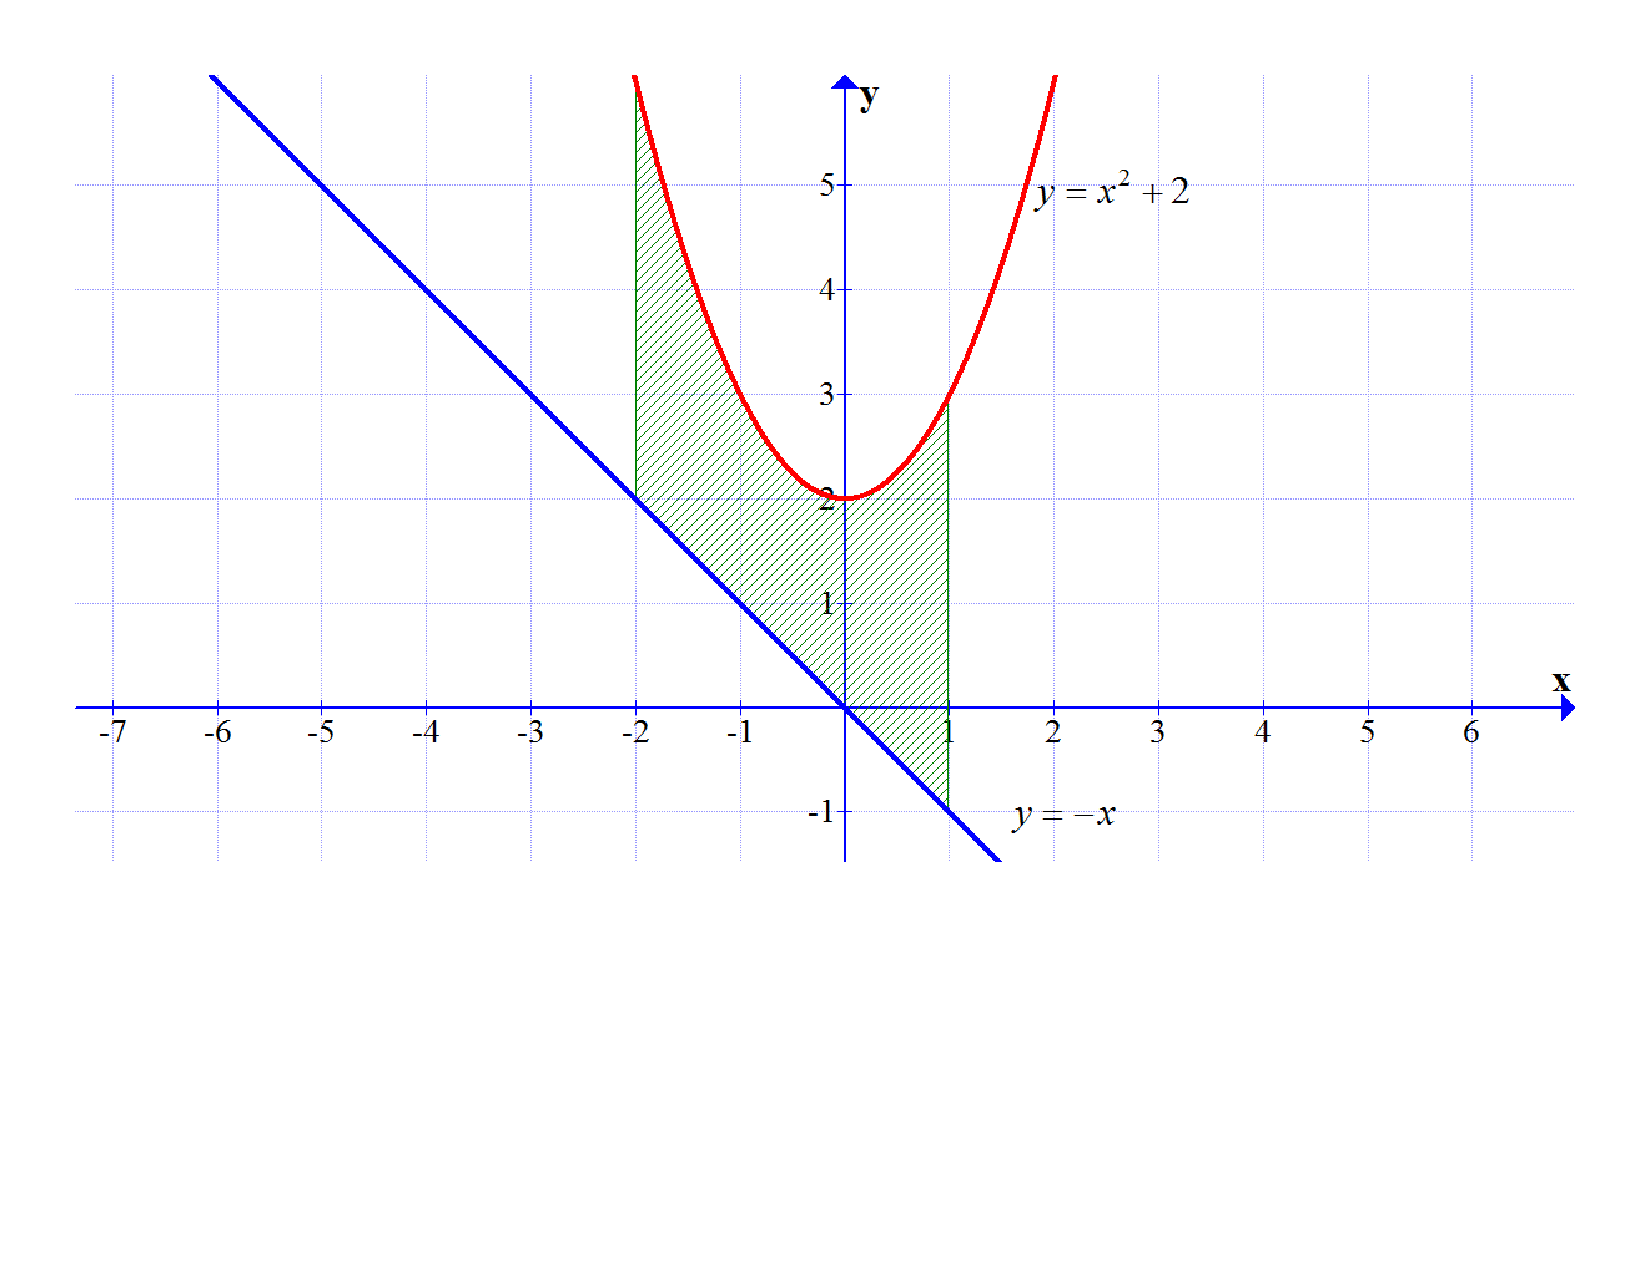
\includegraphics[scale=0.4]{graph1.pdf}

\ifans{\fbox{$A=\frac{15}{2}$}} \fi

\end{center}

\item \text{ }

\begin{center}

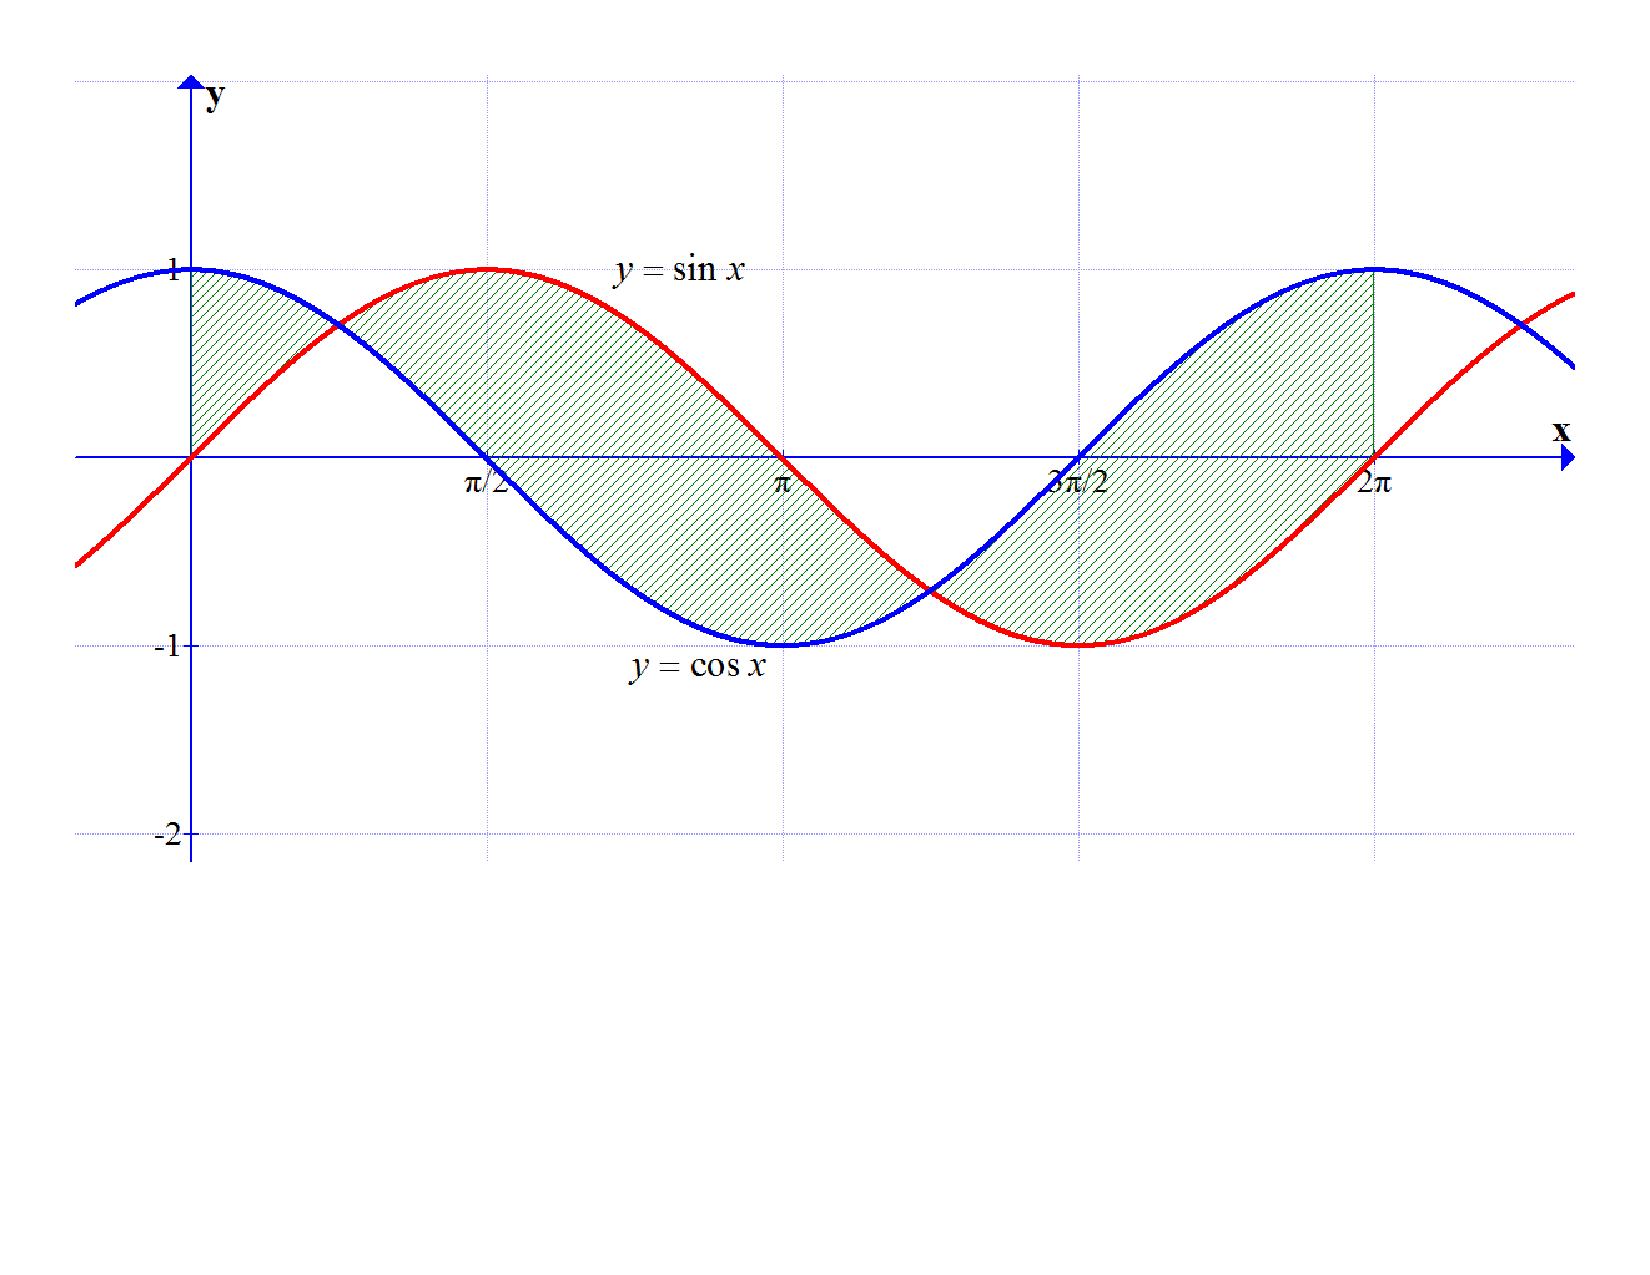
\includegraphics[scale=0.4]{graph2.pdf}

\ifans{\fbox{$A=4\sqrt{2}$}} \fi

\end{center}

\item \text{ }

\begin{center}

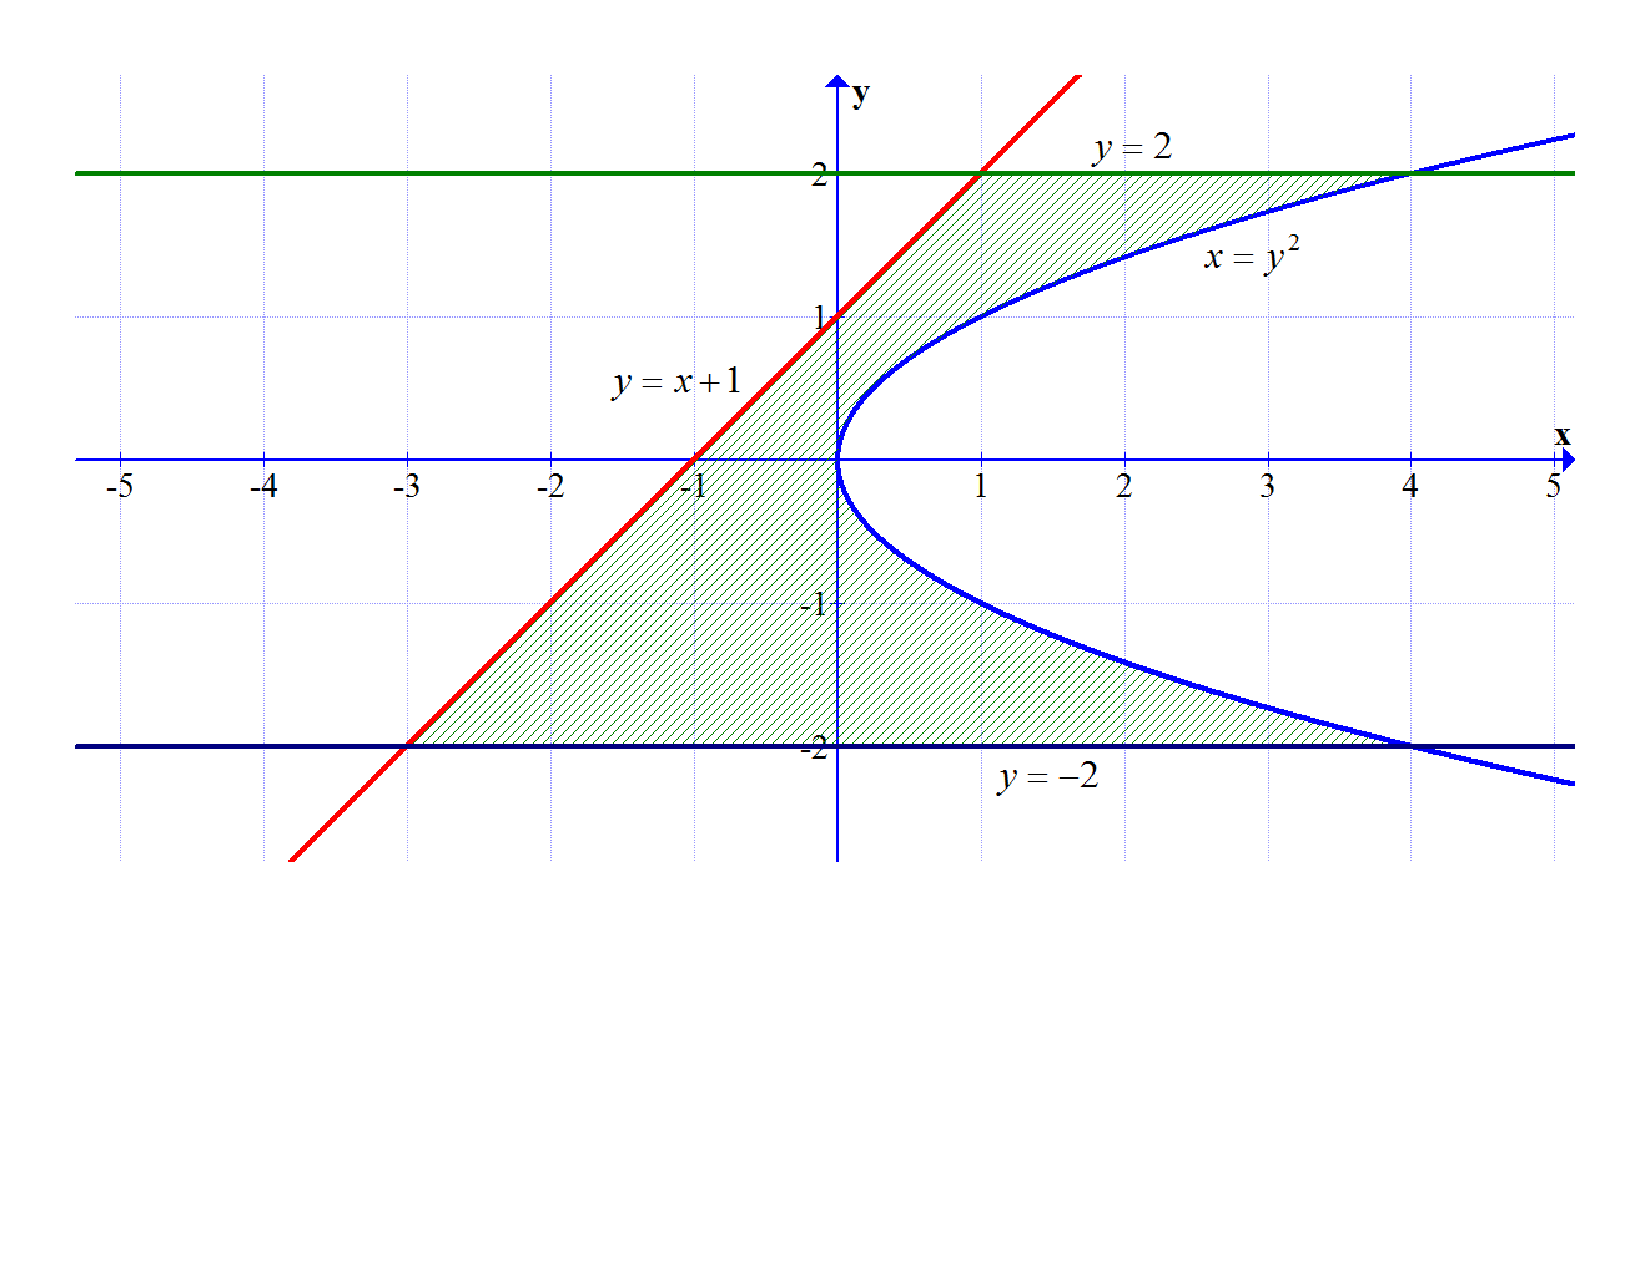
\includegraphics[scale=0.4]{graph4.pdf}

\ifans{\fbox{$A=\frac{28}{3}$}} \fi

\end{center}

\end{enumerate}

\noindent {\bf For problems 5-13, compute the area of the region which is enclosed by the given curves.}

\begin{enumerate}
\setcounter{enumi}{4}

\item $y=4x$, $y=6x^2$

\ifans{\fbox{$\frac{8}{27}$}} \fi

\item $y=2x^2$, $y=x^2+2$

\ifans{\fbox{$\frac{8\sqrt{2}}{3}$}} \fi

\item $y=x^{2/3}$, $y=x^4$, in the first quadrant

\ifans{\fbox{$\frac{2}{5}$}} \fi

\item $y=\frac{1}{x}$, $y=\frac{1}{x^2}$, $x=4$

\ifans{\fbox{$-\frac{3}{4}+2\ln{2}$}} \fi

\item $y=\sin{x}$, $y=2-\sin{x}$, $\frac{\pi}{2}\leq x \leq \frac{5\pi}{2}$

\ifans{\fbox{$4\pi$}} \fi

\item $y=e^{5x}$, $y=e^{8x}$, $x=1$

\ifans{\fbox{$\frac{3}{40}+\frac{1}{8}e^{8}-\frac{1}{5}e^5$}} \fi

\item $x=4-y^2$, $x=y^2-4$

\ifans{\fbox{$\frac{64}{3}$}} \fi

\item $y=x^4$, $y=|x|$

\ifans{\fbox{$\frac{3}{5}$}} \fi

\item $y=x^2$, $y=\frac{2}{x^2+1}$

\ifans{\fbox{$\pi-\frac{2}{3}$}} \fi

\newpage

\item Let $R$ be the region enclosed by $y=x$, $y=8x$, and $y=4$.  

\begin{enumerate}

\item Compute the area of $R$ by evaluating an integral (or integrals) \underline{in terms of $x$}.

\ifans{\fbox{$\int_{0}^{\frac{1}{2}} 7x \,dx + \int_{\frac{1}{2}}^4 (4-x) \,dx= 7$}} \fi

\item Compute the area of $R$ by evaluating an integral (or integrals) \underline{in terms of $y$}.

\ifans{\fbox{$\int_0^4 \frac{7}{8}y \,dy=7$}} \fi

\end{enumerate}

\item Use an integral (or integrals) to compute the area of the triangle in the $xy$-plane which has vertices $(0,0)$, $(2,3)$, and $(-1,6)$.

\ifans{\fbox{$\frac{15}{2}$}} \fi

\item Consider the 2D ice cream cone topped with a delicious scoop of ice cream that is enclosed by $y=6|x|$ and $y=16-x^2$.

\begin{enumerate}

\item Compute the area enclosed within the ice cream cone (including the scoop portion).

\ifans{\fbox{$\frac{104}{3}$}} \fi

\item After a bite is taken from the top, the remaining area is enclosed by $y=6|x|$, $y=16-x^2$, and $y=x^2+12$.  Compute the area of the remaining portion.

\ifans{\fbox{$\frac{104}{3}-\frac{16\sqrt{2}}{3}$}} \fi

\end{enumerate}

\item Consider the region R shown below:

\begin{center}

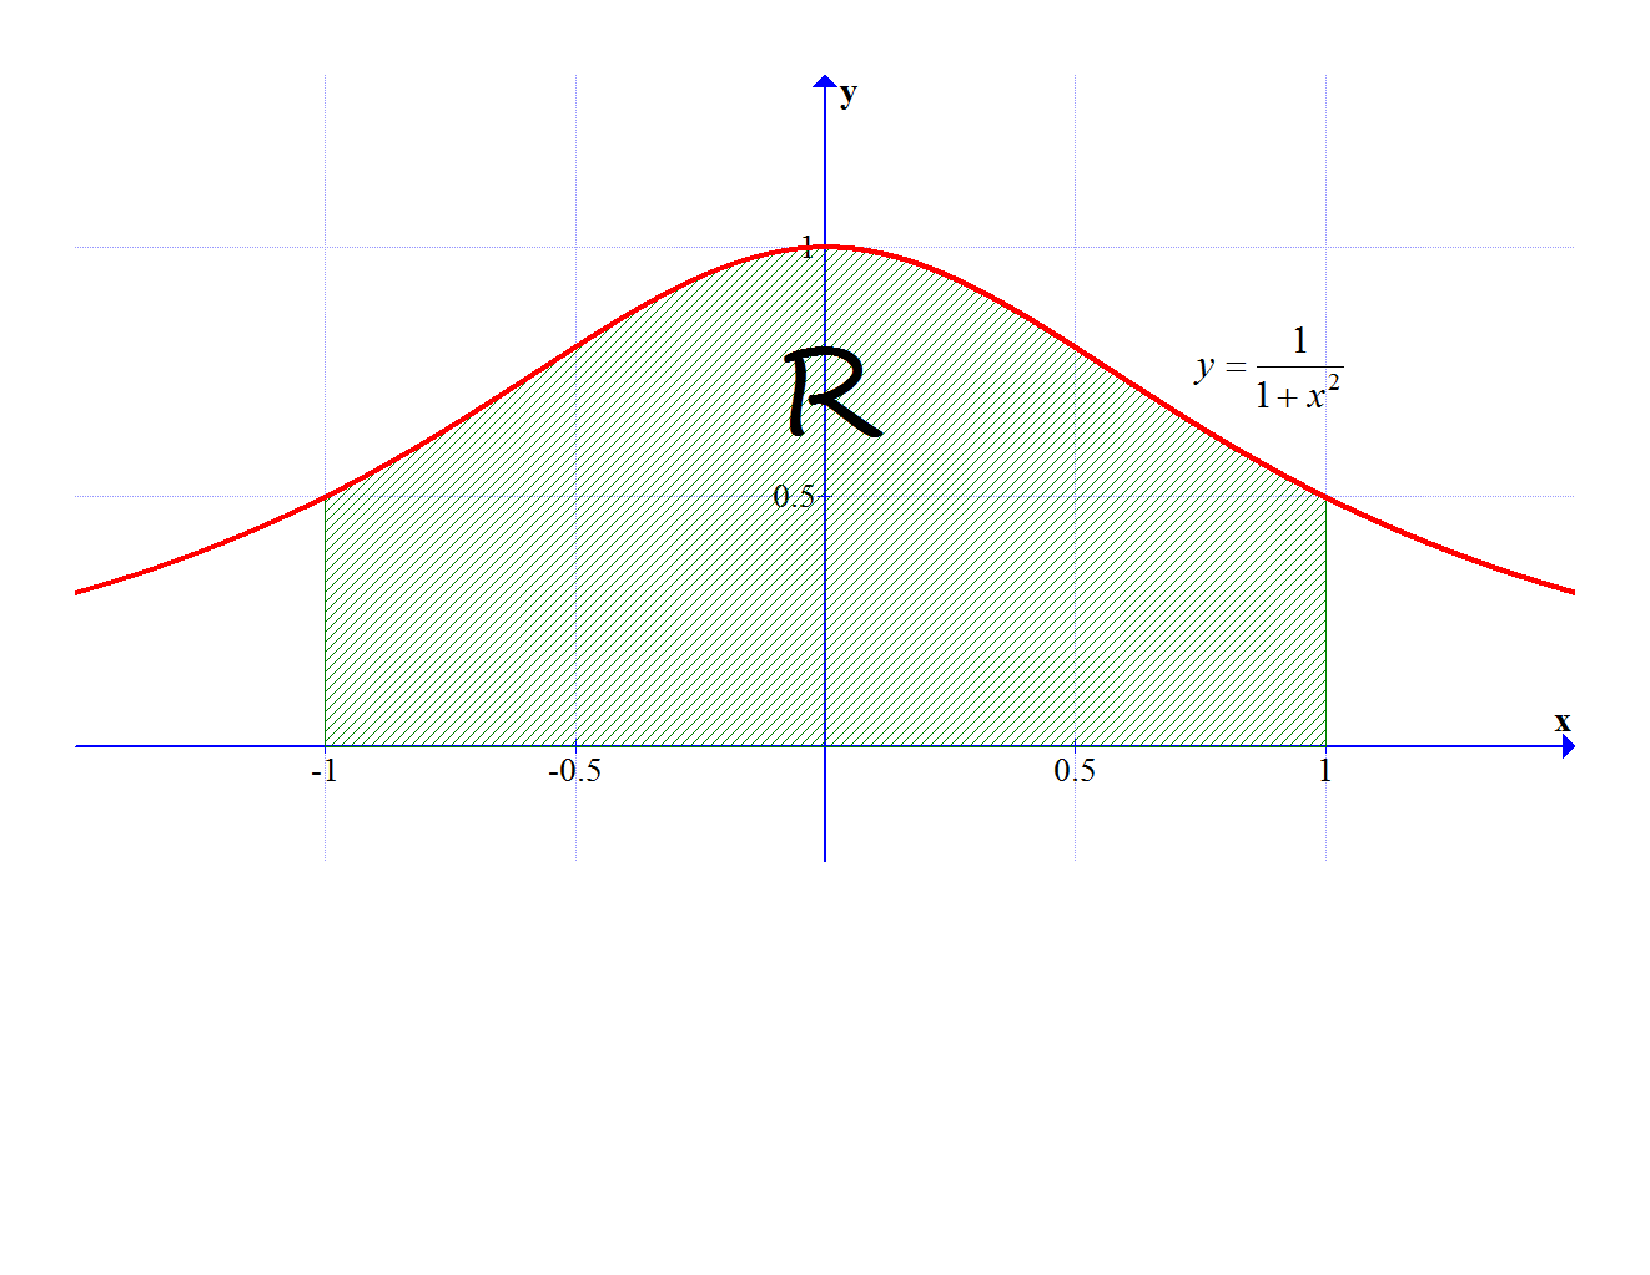
\includegraphics[scale=0.3]{area.pdf}

\end{center}

The area of the region $R$ is equivalent to $\int_{-1}^1 \frac{1}{1+x^2} \,dx$.

\begin{enumerate}

\item Using the substitution $u=\tan^{-1}x$, express the given integral (including the limits of integration) in terms of the variable $u$.

\ifans{\fbox{$\int_{-\frac{\pi}{4}}^{\frac{\pi}{4}} 1 \,du$}} \fi

\item Sketch a region whose area is equivalent to your integral from part (a).  Label this region $S$.

\ifans{\fbox{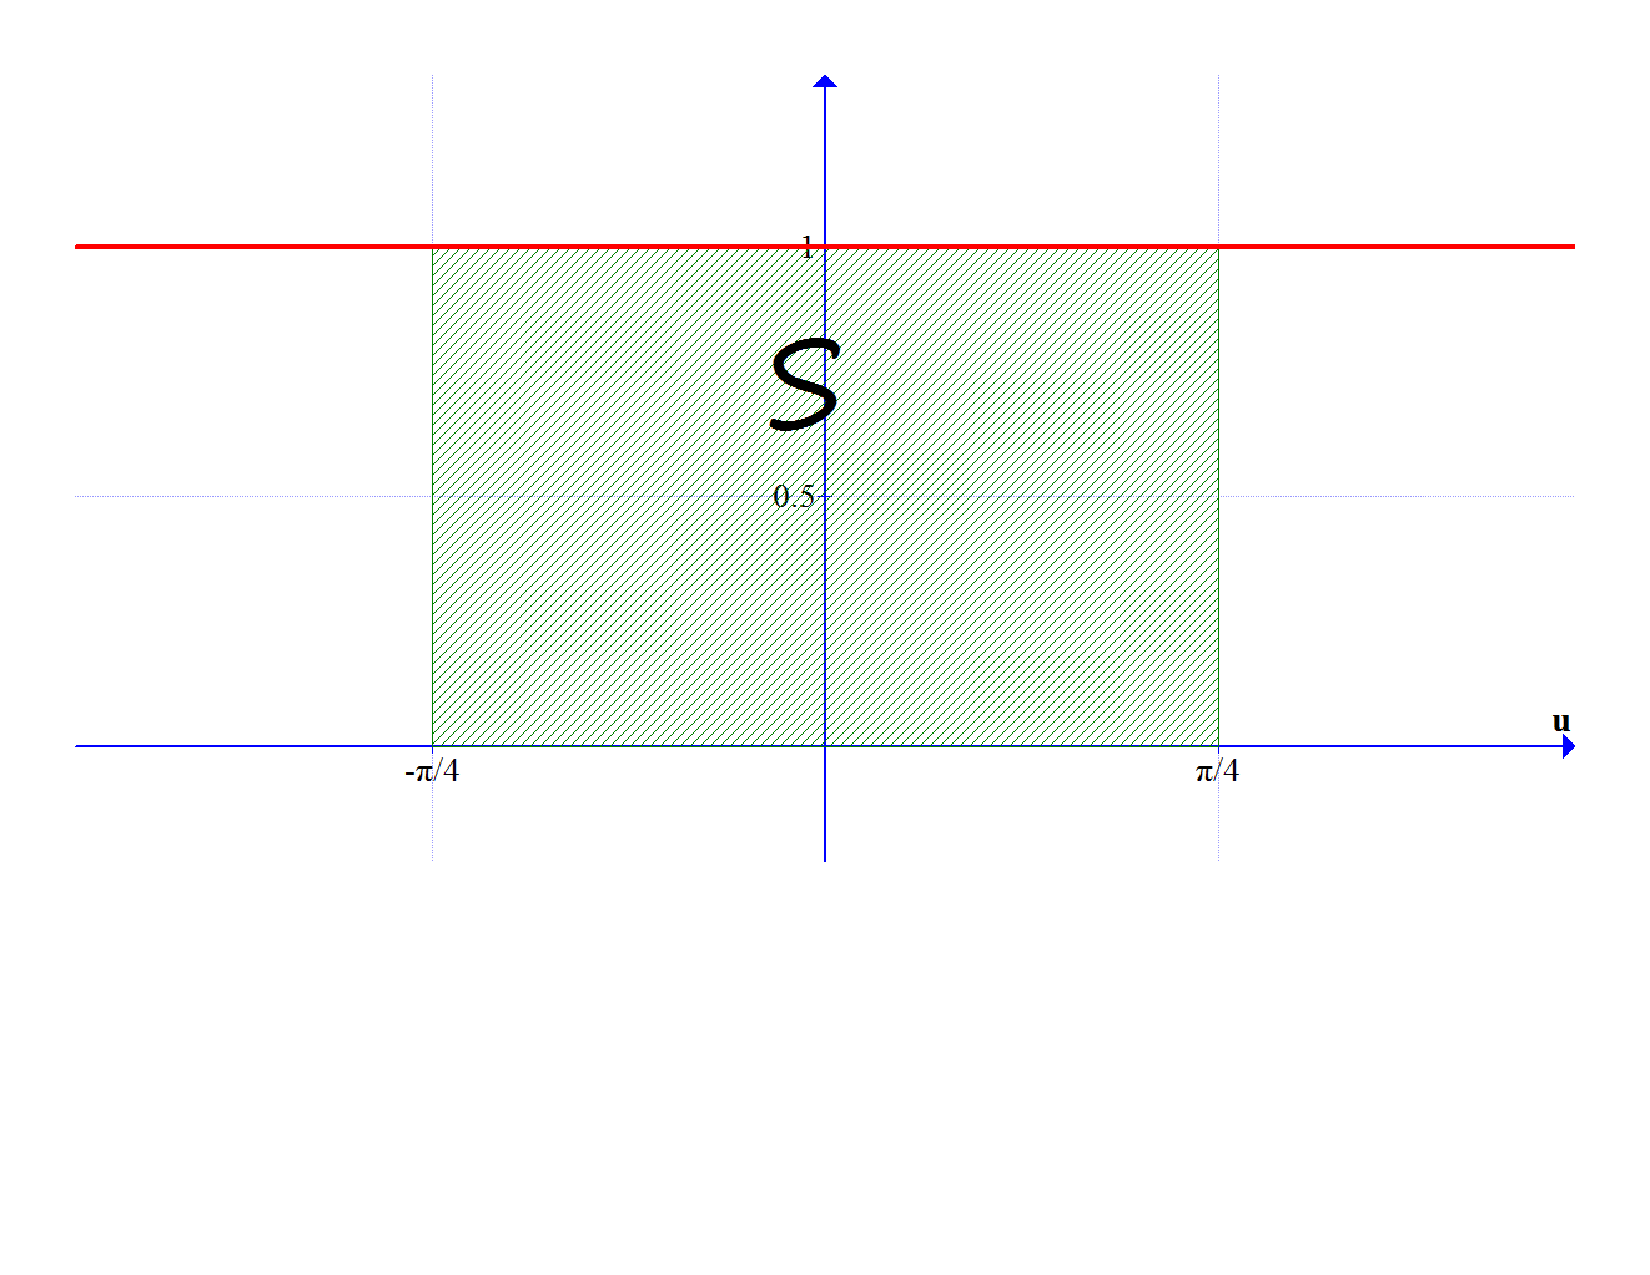
\includegraphics[scale=0.3]{area2.pdf}}} \fi

\item Evaluate the original integral and your integral from part (a).  Conclude that the area of region $R$ is equal to the area of region $S$.

(Note: This is an example of how changing coordinate systems can simplify a problem.  We will discuss this idea more in Math 200 and Math 201.)

\ifans{\fbox{$\frac{\pi}{2}$}} \fi

\end{enumerate}

\end{enumerate}

\end{document}